\documentclass[aspectratio=169]{beamer}


\usepackage[brazil]{babel}
\usepackage[utf8]{inputenc}
\usepackage{algorithm, algpseudocode}
\usepackage{graphicx}
\usepackage{subfig}
\usepackage{multicol}
\usepackage{verbatim}
\usepackage[absolute]{textpos}
\usepackage{todonotes}\presetkeys{todonotes}{inline}{}
\usepackage{minted}
\makeatletter
\renewcommand{\ALG@beginalgorithmic}{\small}
\makeatother

\usetheme[progressbar=foot]{metropolis}

\title{Arquitetura de Computadores}
\subtitle{Reduced Instruction Set Computer: RISC-V}
\date{Última Atualização: \today}
\author{Rodolfo Labiapari Mansur Guimarães}

\institute{
	\textit{rodolfolabiapari@gmail.com} \\
	Lattes: \url{http://goo.gl/MZv4Dc} \\
	Departamento de Computação -- Universidade Federal de Ouro Preto \\
		Ouro Preto - MG -- Brasil }



\begin{document}
\maketitle

\usebackgroundtemplate{
\includegraphics[trim=0 245cm 0 0, width=0.05\textwidth]{img/ufop.jpg}}

\section{Introdução}
\begin{frame}{Introdução ao RISC-V}
	\begin{itemize}
		\item Desenvolver uma CPU requer experiência ao design em várias especialidades:
		\begin{itemize}
			\item Eletrônica Digital, Compiladores e Sistemas Operacionais.
		\end{itemize}

		\item Quando um projeto é baseado de uma série de projetos acadêmicos de design de computadores tem-se então um projeto que abrange vários requisitos.

		\item Foi desenvolvido por profissionais e voluntários entusiastas e com isso obtêm-se como resultado um moderno e de alta qualidade conjunto de instruções para computador de propósito geral, o RISC-V.

		\item Para projetar tal ISA, os autores possuíam vasta experiência em pesquisa na área além de simulação e validação dos design do projeto.

		\item RISC-V é um novo conjunto de instruções de arquitetura com \textbf{propósito geral}.

	\end{itemize}
\end{frame}


\begin{frame}{Introdução ao RISC-V}
	\begin{itemize}
		\item Produzido pelo Computer Science Divison na Universidade da Califórnia, Berkeley, é um \textit{Instruction-Set Architecture} (ISA) \textit{open-source} (BSD)
		\begin{itemize}
			\item Possui várias colaborações de voluntários entusiastas.
		\end{itemize}

		\item É um conjunto \textbf{limpo}, \textbf{modular} com inteiros bases em 32, 64 e 128 bits e várias opções de extensão de instruções como ponto-flutuante, multiplicadores, etc.

		\item Cada usuário demanda que os designers considerem a performance e eficiência energética quando projetar processador
		\begin{itemize}
			\item É um conjunto de fácil implementação comparado a outras alternativas e o projeto possui grande aceitação na indústria de semicondutores.
		\end{itemize}

		\item A meta do projeto RISC-V é criar um conjunto de instruções `universal' que é livre e aberto para todos os usuários, provendo tudo que é necessário para suportar perfeitamente qualquer projeto comercial.
	\end{itemize}
\end{frame}

\begin{frame}{Introdução ao RISC-V}
	\begin{itemize}
		\item Em contraste com a maioria dos ISA disponíveis atualmente, RISC-V é disponibilizado livremente para todos usarem bem como quiserem.
		\begin{itemize}
			\item Incluindo fazer \textit{design}, fabricar e vender os chips e \textit{software} RISC-V.
		\end{itemize}

		\item Não é o primeiro projeto desse porte e \textit{open-souce} a aparecer, mas seu projeto é modelado para ser útil nos dispositivos computacionais mais modernos que vão desde servidores, celulares \textit{high-end} até projetos embarcados de pequeno porte.

		\item Em contraste disso, chips da ARM e MIPS Technologies necessitam de licença para uso de suas patentes
		\begin{itemize}
			\item Também requerem acordos de confidencialidade para uso de seus documentos que citam as vantagens de seus design e conjunto de instruções.
		\end{itemize}

		\item O ISA RISC-V tem sido desenvolvido com o mais pequeno, rápido e mínimo gasto de energia de implementações existente hoje
		\begin{itemize}
			\item Sem sobrecarregar outras partes do seu sistema.
		\end{itemize}

	\end{itemize}
\end{frame}

\begin{frame}{Introdução ao RISC-V - Exemplificação}
	\begin{itemize}
		\item Consideremos um smartphone moderno:
		\begin{itemize}
			\item Possui dúzias de \textit{cores} com diferentes pilhas de \textit{softwares}
			\begin{itemize}
				\item Uma aplicação ARM no CPU;
				\item Uma GPU;
				\item 3 à 5 DSP;
				\item Um \textit{core} de gerenciamento de energia.
			\end{itemize}

			\item Em teoria, todos usam uma variante de um ISA simples e muitos casos, reutilizando \textit{hardware} e \textit{software}.

				\bigskip

			\item RISC-V poderia oferecer uma opção prática para unificar todos esses \textit{cores} num único local.
		\end{itemize}
	\end{itemize}
\end{frame}

\begin{frame}{Introdução ao RISC-V - Propósito}
	\begin{itemize}
		\item Seu propósito de mercado é amplo ao ponto de ser suportado para executar em:
		\begin{itemize}
			\item Microcontroladores que processem imagens, gráficos; ou até mesmo
			\item Processadores de servidores.
		\end{itemize}

		\item Assim, o ISA deve ser consistente em microarquiteturas. É direcionado para ser adequado para quase todo tipo de implementação.
		\begin{itemize}
			\item Desde design Scalar in-order até design out-of-order.
			\item Similarmente, é projetado para ser adequado a quase todas implementações. Desde macros sintetizações em FPGA até projetos totalmente customizados.
		\end{itemize}

		\item Por causa do crescente interesse em aceleração em processamento, \textbf{extensibilidade} do RISC-V é parte essencial da universalidade
		\begin{itemize}
			\item Podendo adicionar módulos, temos uma arquitetura que atende a todos os projetos de \textit{hardware}.
		\end{itemize}

		\item Para ativar as extensões, porções do espaço de codificação de instruções já foram reservados para uso futuro.
	\end{itemize}
\end{frame}

\section{Design do RISC-V}
\begin{frame}{O RISC-V em Termos Gerais}
	\begin{itemize}
		\item RISC-V possui 32 registradores inteiros, e 32 registradores opicionais para ponto flutuante.
		\begin{itemize}
			\item Também existe uma variante RISC-V com 16 registradores inteiros.
		\end{itemize}

		\item Sua memória possui endereçamento de 1 byte.

		\item O assembler usa o registrador x0 como um espaço reservado para fazer manuleio de algumas operações, por exemplo o \texttt{move rx to ry} seria
		\begin{enumerate}
			\item Soma rx com 0: \texttt{add r0 to rx};
			\item Salva o resultado em ry: \texttt{store in ry}.
		\end{enumerate}

		\item Registradores de controle e status também, mas somente o nível de privilégio mais alto (user) que poderá acessá-los para medição de performance.
	\end{itemize}
\end{frame}


\begin{frame}{O RISC-V em Termos Gerais}
	\begin{itemize}
		\item Como todos os outros design de RISCs, RISC-V é um máquina load-store.
		\begin{itemize}
			\item Somente estas duas instruções que acessam a memória principal;
			\item Todas as operações lógico-aritméticas ocorrem entre registradores.
		\end{itemize}

		\item Diferentemente de outros projetos RISC acadêmicos otimizados para simplicidade, o conjunto de instruções do RISC-V é desenvolvido para a praticidade de implementações, com características que aumentam a velocidade computacional enquanto reduz seu curso e energia.

		\item Várias otimizações foram feitas como
		\begin{itemize}
			\item Colocar os bits mais significantes numa posição fixa;
			\item Disposição de bits para reduzir o número de multiplexadores no CPU;
		\end{itemize}

	\end{itemize}
\end{frame}

\begin{frame}{O RISC-V em Termos Gerais}
	\begin{itemize}
		\item Foi projetado para alcançar altos e baixos níveis de velocidade com pouco gasto de energia e eletrônicos.

		\item Todas suas instruções possuem 32 bits. Isso gera simplicidade, mas códigos com mais instruções.

		\item RISC-V, intencionalmente, não possui códigos condicionais, nem mesmo bit de \textit{carry}
		\begin{itemize}
			\item Afirmam que isso pode simplificar o desenvolvimento do CPU, minimizando interações entre instruções.
			\item Construíram operandos de comparação dentro dos \textit{jumps} condicionais.
			\item Não possui \textit{carry} de operações aritméticas complicadas.
			\item Não tem detector ou flag para erros aritméticos, incluindo \textit{overflow}, \textit{underflow} e divisão por 0.
		\end{itemize}
	\end{itemize}
\end{frame}

\begin{frame}{O RISC-V em Termos Gerais}
	\begin{itemize}
		\item Foi desenvolvido para suportar sistema de memória e instruções inteira e ponto flutuante de 32, 64 e 128 bits.

		\item Suas funções load e store pode realizar operações com 16 e 8 bits, mas não operações aritméticas.
		\begin{itemize}
			\item Já as instruções de 64 bits, incluem aritméticas de 32-bits.
		\end{itemize}
	\end{itemize}
\end{frame}

\begin{frame}{Introdução ao RISC-V - Propósito}
	\begin{itemize}
		\item RISC-V provê garantia de funcionamento  para:
		\begin{itemize}
			\item Instruções de inteiros tamanho 32, 64 e 128 bits;
			\item Uma família de extensões opcionais/predefinidas.
		\end{itemize}

		\item Embora alguns processadores disponíveis hoje no mercado sejam amplamente utilizados, eles são:
		\begin{itemize}
			\item Complexos; e
			\item É difícil de ser utilizado para experimentação e uso acadêmico.
		\end{itemize}

		\item Com isso, tendo construído uma arquitetura \textbf{simples} e \textbf{clara}, tem-se então implementações finais \textbf{simplificadas}.
	\end{itemize}
\end{frame}

\section{De Projeto Acadêmico à Item Comercial}
\begin{frame}{O Projeto RISC-V}
	\begin{itemize}
		\item Projeto iniciado em 2010, foi disponibilizado em 2015 e já é utilizado em indústrias de grande porte como Google, Mellanox e Oracle além de grandes centros acadêmicos.

		\item Com isso vários projetos funcionais online já estão disponíveis, usufruindo da permissão de licença BSD.
			\item Um exemplo é o escalar de 5 estágios chamado RISC-V Rocket\footnote{Disponível em: \url{https://github.com/ucb-bar/rocket}} em Scala e para sintetização em chips\footnote{Disponível em: \url{https://github.com/ucb-bar/rocket-chip}}.
	\end{itemize}
\end{frame}


\section{ISA Modular}
\begin{frame}{RISC-V - Extensões}
	\begin{figure}
		\centering
		\label{fig:bi}
		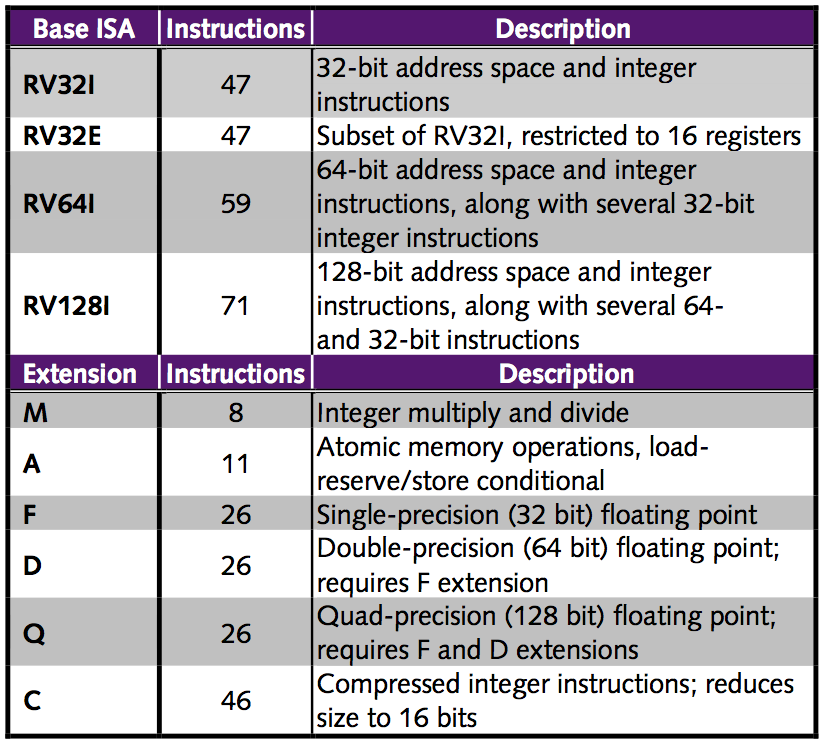
\includegraphics[width=0.6\textwidth]{img/base-instruction.png}
	\end{figure}
\end{frame}

\begin{frame}{Modelo de Instruções}
	\begin{columns}
		\begin{column}{0.58\textwidth}
			\begin{figure}
				\centering
				\label{fig:bi2}
				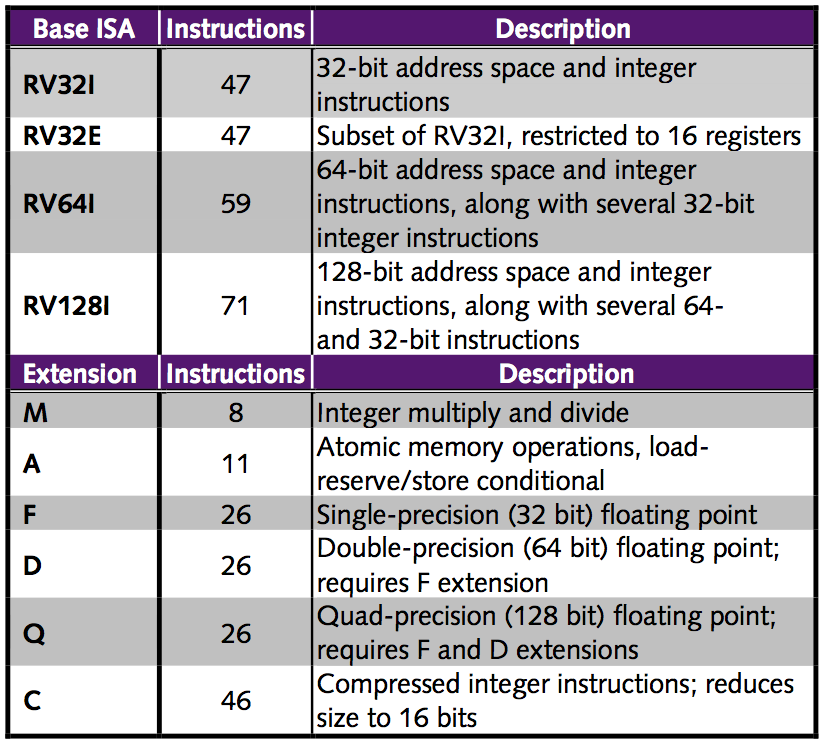
\includegraphics[width=1\textwidth]{img/base-instruction.png}
			\end{figure}
		\end{column}
		\begin{column}{0.55\textwidth}
			\begin{itemize}
				\item O modelo de programação \textbf{RV32I} é escasso. Nele é contido:
				\begin{itemize}
					\item \textit{Program Counter} e 32 registradores inteiros (x0 - x31).
					\item Não contém registrador de retorno sendo este o x1.
				\end{itemize}
				\item As instruções possuem 32 bits possuindo várias combinações de imediatos, operandos e outra especificações.
				\begin{itemize}
					\item O opcode e operando ficam em locais fixos, facilitando o processo de decodificação.
				\end{itemize}
			\end{itemize}
		\end{column}
	\end{columns}
\end{frame}

\begin{frame}{Modelo de Memória}
	\begin{itemize}
		\item Sua memória é endereçada por byte e utiliza-se \textit{little-endian}.
		\item Enquanto outros processadores utilizam complexos instruções e modos de endereçamento, RISC-V usa somente \textit{base}+\textit{offset}.
		\item Podem operar em dados de tamanho 8 (byte), 16 (half-word) ou 32 (word) bits além das opções de sinalização.
	\end{itemize}
\end{frame}

\section{Variantes e Extensões}
\begin{frame}{RISC-V - Variantes}
	\begin{itemize}
		\item Todas as outras variantes do RISC-V são baseadas do \textbf{RV32I}.

			\bigskip

		\item \textbf{RV32E}:
		\begin{itemize}
			\item Possui a meta para ser satisfatório para implementações de \textbf{pequeno porte}.
			\item Sendo um projeto menor, ocupa-se uma pequena porção de área \textit{die}.
			\begin{itemize}
				\item Aumenta o custo/benefício de produção de chips;
				\item Melhora a dissipação de calor por se tratar de um chip com menos área de circuito;
				\item Isso reduz registradores para somente o \textit{Program Counter} e x0-x15.
			\end{itemize}
			\item De resto, RV32E e RV32I são idênticos, com exceção de:
			\begin{itemize}
				\item Suas instruções continuam com tamanho de 32 bits.  Os bits de maior índices são 0.
			\end{itemize}
		\end{itemize}

		\item \textbf{RV64I} e \textbf{RV128I}:
		\begin{itemize}
			\item Simples extensões de 64 e 128 bits.
			\item Aumentam o espaço de endereço e estende os registradores de 32 para o tamanho apropriado.
			\item Essa extensão introduz novas instruções que operam com dados menores como 32 e 64 bits.
		\end{itemize}
	\end{itemize}
\end{frame}

\begin{frame}{RISC-V - Extensões - Multiplicação}
	\begin{columns}
		\begin{column}{0.58\textwidth}
			\begin{figure}
				\centering
				\label{fig:bi2}
				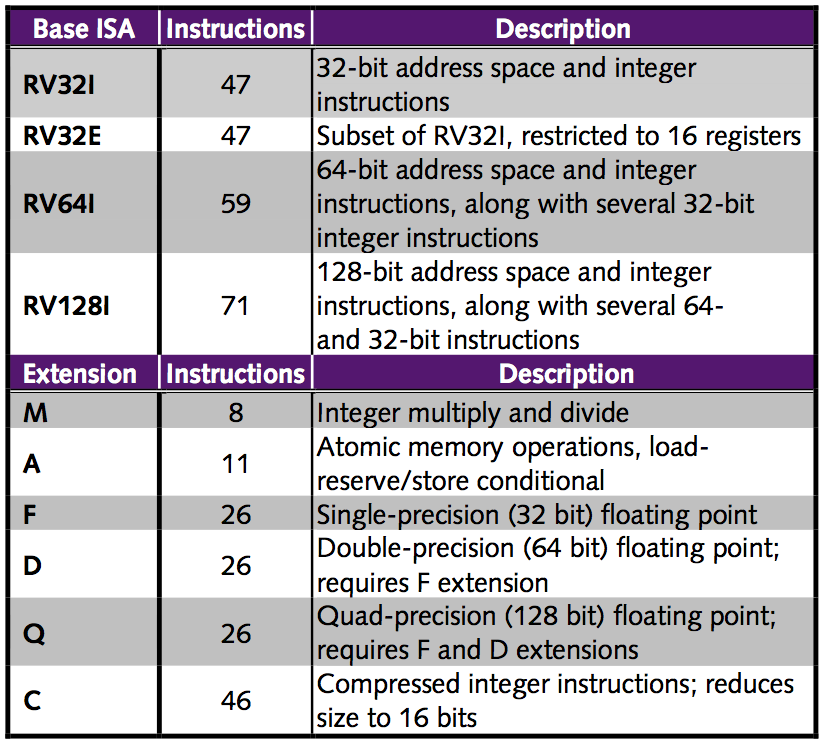
\includegraphics[width=1\textwidth]{img/base-instruction.png}
			\end{figure}
		\end{column}
		\begin{column}{0.55\textwidth}
			\begin{itemize}
				\item \textbf{Multiplicação M}:
				\begin{itemize}
					\item Adiciona 4 instruções de multiplicação, duas de divisão, e duas de manipulação de restos.
					\item A base é indicada pela base do ISA.
					\item A divisão por 0, por exemplo, não causa interrupção, mantendo a simplicidade.
				\end{itemize}
			\end{itemize}
		\end{column}
	\end{columns}
\end{frame}

\begin{frame}{RISC-V - Extensões - Sincronização}
	\begin{columns}
		\begin{column}{0.58\textwidth}
			\begin{figure}
				\centering
				\label{fig:bi2}
				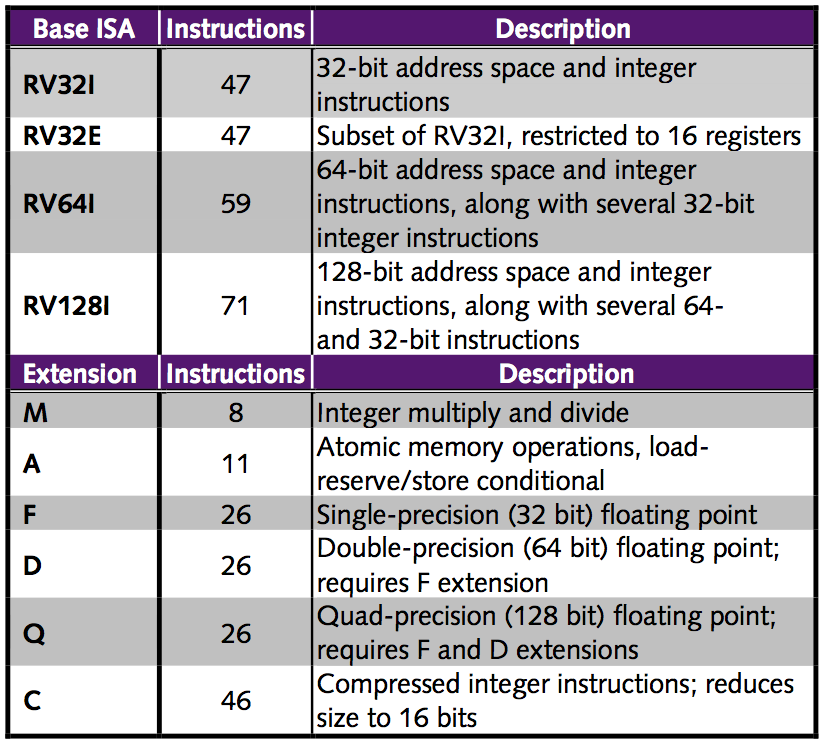
\includegraphics[width=1\textwidth]{img/base-instruction.png}
			\end{figure}
		\end{column}
		\begin{column}{0.55\textwidth}

			\begin{itemize}
				\item \textbf{Sincronização A}:
				\begin{itemize}
					\item Adiciona 11 instruções de sincronização visando consistência e atomicidade da operação.
					\item São divididos em dois grupos: \textit{Load} Reserved e \textit{Store} Conditional para operações atômicas na memória.
				\end{itemize}

			\end{itemize}
		\end{column}
	\end{columns}
\end{frame}

\begin{frame}{RISC-V - Extensões - Ponto Flutuante}
	\begin{columns}
		\begin{column}{0.58\textwidth}
			\begin{figure}
				\centering
				\label{fig:bi2}
				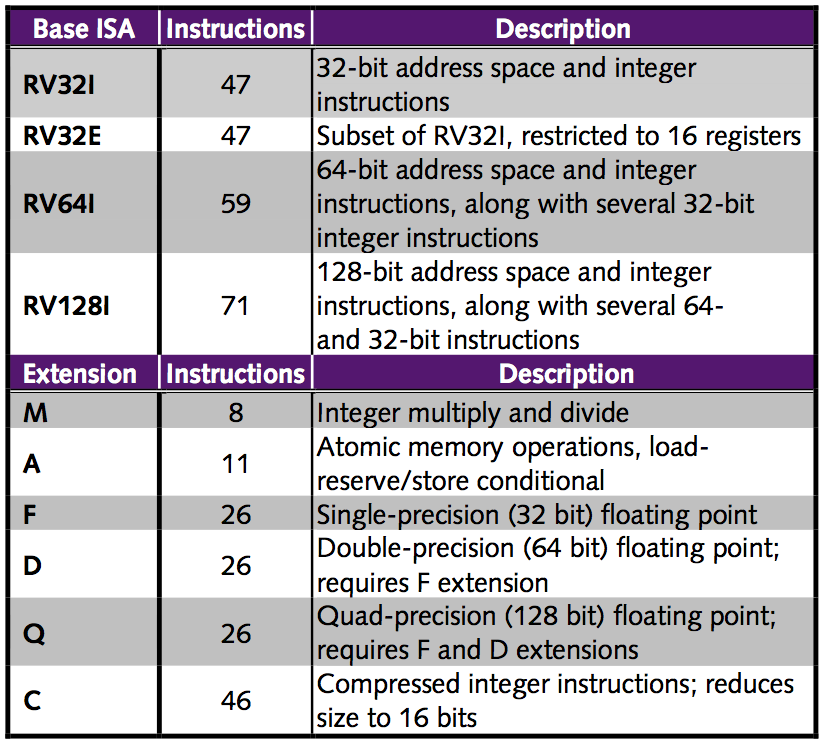
\includegraphics[width=1\textwidth]{img/base-instruction.png}
			\end{figure}
		\end{column}
		\begin{column}{0.55\textwidth}

			\begin{itemize}
				\item Possui três extensões diferentes:
				\begin{itemize}
					\item Precisão simples (\textbf{F}), Precisão Dupla (\textbf{D}) e quádrupla precisão (\textbf{Q}).
				\end{itemize}
				\item A extensão F é pré-requisito para D, que é pré-requisito para Q.
				\item Introduz também 32 registradores de ponto flutuante (f0-f31) de tamanho 32 bits.
				\item Registrador de 5 bits para exceções.
				\begin{itemize}
					\item Exceções não geram interrupções. Devem ser verificadas por meio de consultas.
				\end{itemize}
				\item As instruções \textit{load}-\textit{store} usam o mesmo endereçamento \textit{base}+\textit{offset}.
			\end{itemize}
		\end{column}
	\end{columns}
\end{frame}

\begin{frame}{RISC-V - Extensões - Compressão de Tamanho de Código}
	\begin{columns}
		\begin{column}{0.58\textwidth}
			\begin{figure}
				\centering
				\label{fig:bi2}
				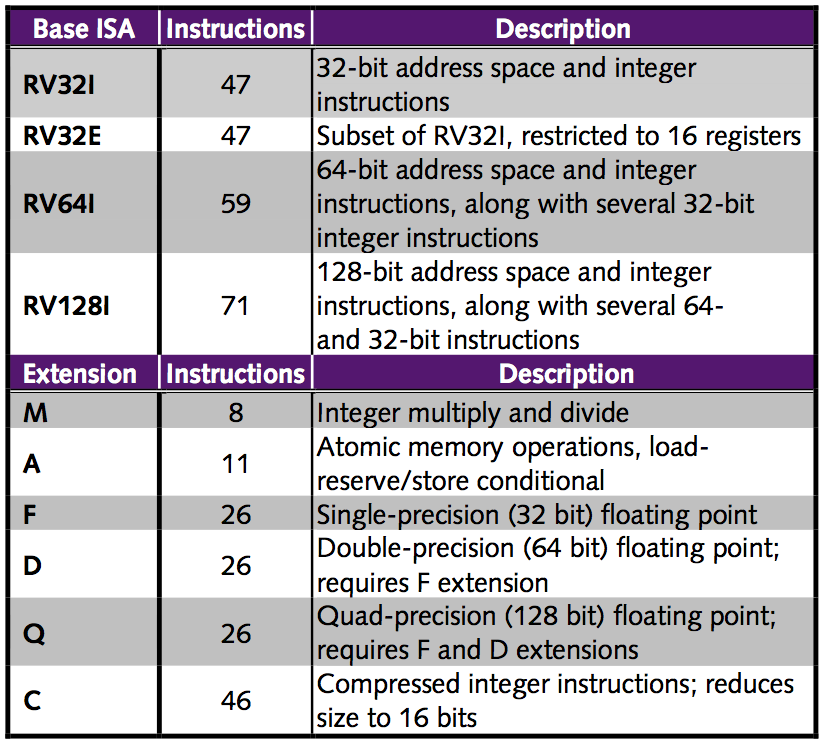
\includegraphics[width=1\textwidth]{img/base-instruction.png}
			\end{figure}
		\end{column}
		\begin{column}{0.55\textwidth}
			\begin{itemize}
				\item A última extensão \textbf{C} não adiciona nenhum outra função, mas, ao invés disso, \textbf{codifica} as instruções inteiras para \textbf{salvar espaço} e com isso reduzir o tamanho do \textit{footprint}.
				\item É disponível para bases inteiras, bem como \textit{load} e \textit{store} para pontos flutuantes.
				\item Cria-se instruções compressadas em 16 bit
				\begin{itemize}
					\item Basicamente, cada função compactada é mapeada diretamente à instrução real.
				\end{itemize}
				\item Possui algumas restrições para a compressão sobre o formato dos operandos.
			\end{itemize}
		\end{column}
	\end{columns}
\end{frame}

\begin{frame}{RISC-V - Extensões - Compressão de Tamanho de Código}
	\begin{columns}
		\begin{column}{0.58\textwidth}
			\begin{figure}
				\centering
				\label{fig:bi2}
				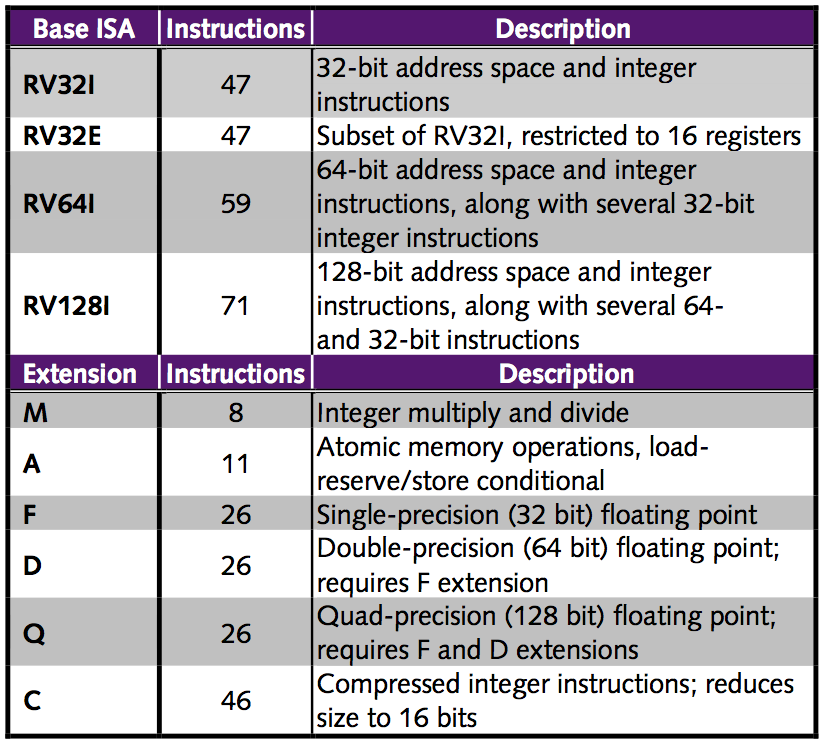
\includegraphics[width=1\textwidth]{img/base-instruction.png}
			\end{figure}
		\end{column}
		\begin{column}{0.55\textwidth}
			\begin{itemize}
				\item O propósito de reduzir o tamanho do código binário, energia e custo para pequenos computadores, é visando sistemas embarcados.

				\item Pesquisas com \textbf{C} mostram que um código 20\% menor que um x86 e MIPS Comprimido e 2\% maior que um ARM Thumb-2.
			\end{itemize}
		\end{column}
	\end{columns}
\end{frame}

\section{Níveis de Privilégios}
\begin{frame}{RISC-V - Níveis de Privilégios}
	\begin{itemize}
		\item Existe 4 níveis de privilégios:
		\begin{itemize}
			\item User (\textbf{U});
			\item Supervisor (\textbf{S});
			\item Hypervisor (\textbf{H}); e
			\item Machine (\textbf{M}).
		\end{itemize}

		\item Para reduzir o custo de uma implementação mínima, somente o \textit{machine} é requerido.
		\begin{itemize}
			\item Entretanto, todos os 4 privilégios são suportados.
			\item Quando suportados, é possível até executar o Linux.
		\end{itemize}
	\end{itemize}
\end{frame}

\section{O Ecossistema Open-Source}
\begin{frame}{RISC-V - O Ecossistema do Projeto}
	\begin{itemize}
		\item O projeto ainda está incompleto, mas as especificações já mostram que é bastante promissor.
		\item Sua arquitetura é mais fácil de ser implementada do que um ARM, por exemplo:
		\begin{itemize}
			\item Pela sua simplicidade em:
			\begin{itemize}
				\item Decodificar códigos;
				\item Nos modos de endereçamento.
			\end{itemize}
			\item Omite instruções complexas;
			\item Tudo isso com \textbf{metade} do tamanho de projeto de um ARM \textit{core}.
		\end{itemize}
		\item É considerado como a técnica mais \textbf{promissora} em flexibilidade de extensões customizadas combinado com arquitetura de propósito geral.
	\end{itemize}
\end{frame}

\begin{frame}{RISC-V - O Ecossistema do Projeto}
	\begin{itemize}
		\item Extensões potenciais do RISC-V incluem novos tipos como
		\begin{itemize}
			\item Extensões Cray-style vector;
			\item Memória Transacional; e
			\item Manipulação de bit.
		\end{itemize}

		\item Outras extensões são disponibilizadas para obter melhor desempenho, mas requerem cadeias de ferramentas e limitam a portabilidade de \textit{software}.

	\end{itemize}
\end{frame}

\begin{frame}{RISC-V - O Ecossistema do Projeto}
	\begin{itemize}
		\item O ecossistema RISC-V ainda está nos estágios iniciais
		\begin{itemize}
			\item Um \textbf{Linux} 4.1 foi sido portado para o projeto RISC-V
			\begin{itemize}
				\item E um Linux Embarcado (\textbf{Yocto}) também foi disponibilizado.
			\end{itemize}
			\item Várias ferramentas do RISC-V incluem \textbf{compiladores} GCC, LLVM e Clang, GDB, uma suite de \textbf{verificação} e \textbf{simuladores}.
		\end{itemize}
		\item Oferece todos os recursos básicos de um RISC com implementações simplificadas, reduzindo a \textit{die area} e potencialmente, energia consumida por ele.
		\item Comparado os dois modelos mais populares (ARM e x86)
		\begin{itemize}
			\item Oferece uma considerável área de circuito não utilizada em placa deixando o projeto menos custoso;
			\item Permite a adição de extensões customizadas ou não.
			\item É um projeto \textit{open-source}.
		\end{itemize}
	\end{itemize}
\end{frame}

\section{Adotantes do Projeto}
\begin{frame}{RISC-V - Adotantes do Projeto}
	\begin{itemize}
		\item Um número de organizações comerciais planejam suportar o RISC-V Foundation
		\begin{itemize}
			\item Bluespec, Inc., Google, Hewlett Packard Enterprise (HPE), Lattice Semiconductor, Mellanox Technologies, Microsemi, Oracle e Rambus Cryptography Research.
		\end{itemize}

		\item O Instituto Indiano de Tecnologia Madras estão desenvolvendo 6 RISC-V \textit{open-source} para 6 tipos de usuários diferentes.
		\begin{itemize}
			\item De um pequeno CPU 32 bit para IoT até largos computadores de 64 bit concebido para computadores em escala de de armazenamento.
		\end{itemize}

		\item lowRISC é um projeto sem fins lucrativos que visa implementar um sistema \textit{open-source} num \textit{System on Chip} (SoC) baseado num RISC-V de 64 bits.
	\end{itemize}
\end{frame}

\begin{frame}{RISC-V - Adotantes do Projeto}
	\begin{itemize}
		\item O Laboratório de Computação, na Universidade de Cambridge, em colaboração com o FreeBSD Project, tem suportado o sistema operacional FreeBSD para o RISC-V 64-bit.

		\item ETH Zurich e a Universidade de Bologna têm desenvolvido em cooperação um System on Chip (SoC) de baixa energia usando RISC-V.

		\item Um dos fundadores do Adapteva planeja usar RISC-V como sucessor para o seu produto acelerador multicore.

		\item Nvidia planeja usá-lo para substituir a linha de processadores Falcon em suas placas gráficas GeForce.
	\end{itemize}
\end{frame}

\maketitle

%\section{Bibliografia}

\bibliographystyle{abbrv}
\bibliography{sbc-template}

\maketitle

\end{document}
